\documentclass{ximera}

\input{../preamble.tex}

\title[Dig-In:]{Quadric surfaces}

\begin{document}
\begin{abstract}
  We will get to know some basic quadric surfaces.
\end{abstract}
\maketitle

As we have seen, if we look at the set of points that satisfy an
equation
\[
F(x,y,z)=0
\]
where $F:\R^3\to\R$, we obtain a surface in $\R^3$. A basic class of
surfaces are the \textit{quadric surfaces}.

\begin{definition}
A \dfn{quadric surface} in $\R^3$ is a surface of the form
\[
Ax^2 + By^2 + Cz^2 + Dxy + Exz+ Fyz + Gx + Hy + I z + J = 0
\]
where $A$, $B$, $C$, $D$, $E$, $F$, $G$, $H$, $I$, and $J$ are
constants and at least one of $A$, $B$, $C$, $D$, $E$, or $F$ are
nonzero.
\end{definition}

\begin{warning}
  Do not confuse a \textit{quadric} with a quadratic, or quartic, as
  these are different beasts entirely.
\end{warning}

We will be interested in a special class of quadric surfaces, those of
the form:
\[
z = Ax^2 + By^2 + C xy + D
\]
Quadric surfaces of this form are those that arise naturally when
computing the Taylor polynomial of a surface $z=F(x,y)$ at a point
$\vec{c}$ where
\[
F^{(1,0)}(\vec{c}) = 0 = F^{(0,1)}(\vec{c})
\]
Why are we doing this?
\begin{quote}
  \textbf{Understanding quadric surfaces will help us find extrema of surfaces.}
\end{quote}

In what follows, we will study each shape by considering the
\textit{trace}.

\begin{definition}
  The \dfn{trace} of a surface is the intersections of
  a surface with a plane parallel to a coordinate plane.
\end{definition}

Let's get to it.


\section{Elliptic paraboloids}

An elliptic paraboloid is a surface with graph:
\begin{image}
  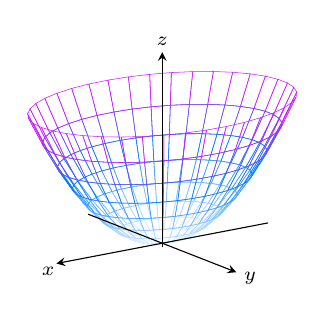
\begin{tikzpicture}
    \begin{axis}%
      [width=175pt,tick label style={font=\scriptsize},axis on top,
	axis lines=center,
	view={145}{20},
	name=myplot,
	xtick=\empty,
	ytick=\empty,
	ztick=\empty,
	ymin=-2.5,ymax=2.5,
	xmin=-3.5,xmax=3.5,
	zmin=-.1, zmax=5.5,
	every axis x label/.style={at={(axis cs:\pgfkeysvalueof{/pgfplots/xmax},0,0)},xshift=-3pt,yshift=-3pt},
	xlabel={\scriptsize $x$},
	every axis y label/.style={at={(axis cs:0,\pgfkeysvalueof{/pgfplots/ymax},0)},xshift=5pt,yshift=-2pt},
	ylabel={\scriptsize $y$},
	every axis z label/.style={at={(axis cs:0,0,\pgfkeysvalueof{/pgfplots/zmax})},xshift=0pt,yshift=4pt},
	zlabel={\scriptsize $z$},
        colormap/cool
      ]
      
      \addplot3[domain=0:360,y domain=0:2,color=black!40,mesh,samples=40,samples y=10,very thin,z buffer=sort] ({2*cos(x)*y},{sin(x)*y},{y^2});
    \end{axis}
  \end{tikzpicture}
\end{image}
and equation:
\[
z=\pm\frac{x^2}{a^2}\pm\frac{y^2}{b^2}
\]
To understand this surface better consider the trace when:
\begin{itemize}
  \item $x=d$, in this case we now have $z = \pm\frac{d^2}{a^2} \pm
    \frac{y^2}{b^2}$, a parabola.
  \item $y=d$, in this case we now have $z = \pm\frac{x^2}{a^2} \pm
    \frac{d^2}{b^2}$, a parabola.
  \item $z=d$, in thisi case we now have $d = \pm\frac{x^2}{a^2} \pm
    \frac{y^2}{b^2}$, an ellipse.
\end{itemize}
\begin{image}
  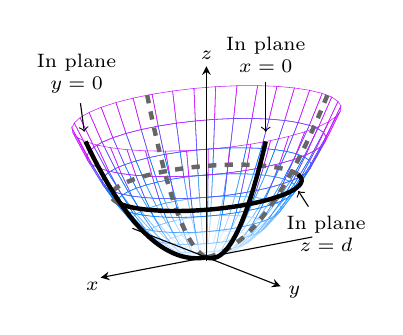
\begin{tikzpicture}
    \begin{axis}%
      [width=175pt,tick label style={font=\scriptsize},axis on top,
	axis lines=center,
        clip=false,
	view={145}{20},
	name=myplot,
	xtick=\empty,
	ytick=\empty,
	ztick=\empty,
	ymin=-2.5,ymax=2.5,
	xmin=-3.5,xmax=3.5,
	zmin=-.1, zmax=5.5,
	every axis x label/.style={at={(axis cs:\pgfkeysvalueof{/pgfplots/xmax},0,0)},xshift=-3pt,yshift=-3pt},
	xlabel={\scriptsize $x$},
	every axis y label/.style={at={(axis cs:0,\pgfkeysvalueof{/pgfplots/ymax},0)},xshift=5pt,yshift=-2pt},
	ylabel={\scriptsize $y$},
	every axis z label/.style={at={(axis cs:0,0,\pgfkeysvalueof{/pgfplots/zmax})},xshift=0pt,yshift=4pt},
	zlabel={\scriptsize $z$},colormap/cool
      ]
      
      \addplot3[domain=0:360,y domain=0:2,mesh,samples=40,samples y=10,very thin,z buffer=sort] ({2*cos(x)*y},{sin(x)*y},{y^2});
      
      \addplot3[domain=170:360,dashed,ultra thick,smooth,samples y=0,black!60,%surf,%fill=white,
        samples=30,] ({2*cos(x)*sqrt(2)},{sin(x)*sqrt(2)},{2});

      \addplot3[domain=-2:0,dashed,ultra thick,smooth,samples y=0,black!60,%surf,%fill=white,
        samples=30,] ({2*x},{0},{x^2});

      \addplot3[domain=-2:0,dashed,ultra thick,smooth,samples y=0,black!60,%surf,%fill=white,
        samples=30,] ({0},{x},{x^2});
      
      \addplot3[domain=0:170,ultra thick,smooth,samples y=0,black,%surf,%fill=white,
        samples=30,] ({2*cos(x)*sqrt(2)},{sin(x)*sqrt(2)},{2});
      
      \addplot3[domain=0:2,ultra thick,smooth,samples y=0,black,%surf,%fill=white,
        samples=30,] ({2*x},{0},{x^2});

      \addplot3[domain=0:2,ultra thick,smooth,samples y=0,black,%surf,%fill=white,
          samples=30,] ({0},{x},{x^2});
      
        \draw (axis cs:4.3,0,6) node[align=center] (A1) {\scriptsize In plane\\[-4pt] \scriptsize $y=0$};
        \draw (axis cs:4,0,4) node (A2) {};
        \draw [->](A1)--(A2);
        
        \draw (axis cs:0,2,6.5) node[align=center] (B1) {\scriptsize In plane\\[-4pt] \scriptsize $x=0$};
        \draw (axis cs:0,2,4) node (B2) {};
        \draw [->](B1)--(B2);

        \draw (axis cs:-2,2,1) node[align=center] (C1) {\scriptsize In plane\\[-4pt] \scriptsize $z=d$};
        \draw (axis cs:-2.83,0,2) node [below] (C2) {};
        \draw [->](C1)--(C2);
        %\foreach \z in {-6.28,-4.71,-1.57,1.57,6.28}
        %{\addplot3[domain=-2:2,,thick,smooth,samples y=0,{\colortwo},%surf,%fill=white,
        %samples=30,] ({sin(deg(\z))},{x},{\z});
        %}
    \end{axis}
  \end{tikzpicture}
\end{image}
\[
\begin{array}{ccc}
\textbf{Plane}  & & \textbf{Trace} \\ \hline
x=d & & \text{Parabola} \\
y=d & & \text{Parabola}\\
z=d & & \text{Ellipse}
\end{array}
\]




\section{Hyperbolic paraboloids}

A hyperbolic paraboloid is a surface with graph:
\begin{image}
  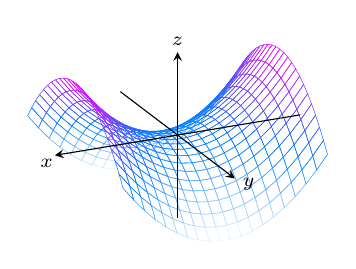
\begin{tikzpicture}[>=stealth]
    \begin{axis}%
      [width=175pt,tick label style={font=\scriptsize},axis on top,
	axis lines=center,
	view={155}{30},
	name=myplot,
	xtick=\empty,
	ytick=\empty,
	ztick=\empty,
	ymin=-1.2,ymax=1.2,
	xmin=-1.2,xmax=1.2,
	zmin=-1.2, zmax=1.2,
	every axis x label/.style={at={(axis cs:\pgfkeysvalueof{/pgfplots/xmax},0,0)},xshift=-3pt,yshift=-3pt},
	xlabel={\scriptsize $x$},
	every axis y label/.style={at={(axis cs:0,\pgfkeysvalueof{/pgfplots/ymax},0)},xshift=5pt,yshift=-2pt},
	ylabel={\scriptsize $y$},
	every axis z label/.style={at={(axis cs:0,0,\pgfkeysvalueof{/pgfplots/zmax})},xshift=0pt,yshift=4pt},
	zlabel={\scriptsize $z$},
        colormap/cool
      ]

      \addplot3[domain=-1:1,smooth,y domain=-1:1,mesh,samples=20,samples y=25,very thin,z buffer=sort] ({x},{y},{x^2-y^2});
    \end{axis}
  \end{tikzpicture}
\end{image}
and equation:
\[
z=\pm\frac{x^2}{a^2}\mp\frac{y^2}{b^2}
\]
To understand this surface better consider the trace when:

\end{document}

\[
\begin{array}{ccc}
\textbf{Plane}  & & \textbf{Trace} \\ \hline
$x=d$ & & Parabola\\
$y=d$ & & Parabola\\
$z=d$ & & Hyperbola
\end{array}
\]

\myincludegraphics[scale=1.25,trim=1mm 5mm 3mm 2mm,clip]{figures/figquadric_hyp_parb}
\end{minipage}
\begin{minipage}[t]{.4\linewidth}
\vskip0pt
\myincludegraphics[scale=1.25,trim=1mm 5mm 3mm 2mm,clip]{figures/figquadric_hyp_parc}
\end{minipage}

\vskip2\baselineskip
\begin{minipage}[t]{.75\linewidth}
The parabolic traces will open along the axis of the one variable that is raised to the first power.
\index{quadric surface!gallery|)}\index{quadric surface!hyperbolic paraboloid}

\end{minipage}
\end{minipage}


\begin{sageCell}
var ('x y z')
A = 3
B = 4
C = 1
implicit_plot3d(A*x^2+B*y^2-C*z^2==1,
                (x,-6,6), 
                (y,-6,6), 
                (z,-6, 6), 
                axes="true")
\end{sageCell}

\end{document}
